\chapter{Results}
\section{DBSCAN Results}

Using the selected value of \(\varepsilon=4.5\) and
\(\texttt{min\_samples}=20\),
DBSCAN identified one large cluster and a set of noise observations.

\begin{table}[H]
\centering
\begin{tabular}{lcc}
\hline
Cluster & Accounts & Proportion \\
\hline
Cluster 0 & 1777 & 97.3\% \\
Noise (-1) & 49 & 2.7\% \\
\hline
\end{tabular}
\caption{DBSCAN cluster sizes.}
\end{table}
\begin{table}[H]
\centering
\small
\begin{tabular}{lcc}
\hline
Feature & Cluster 0 & Noise (-1) \\
\hline
Transactions per active day & 2.858 & 12.551 \\
Log outgoing amount per span day & 3.927 & 5.812 \\
Outgoing transaction ratio & 0.747 & 0.717 \\
Outgoing amount ratio & 0.507 & 0.594 \\
Off-hours ratio & 0.619 & 0.592 \\
Weekend ratio & 0.196 & 0.171 \\
Mean-to-median amount ratio & 0.622 & 0.625 \\
P90-to-median amount ratio & 15.320 & 484.870 \\
Max-to-median amount ratio & 363.317 & 5474.357 \\
Near pass-through ratio (1h) & 0.018 & 0.144 \\
Near pass-through ratio (24h) & 0.061 & 0.253 \\
One-in-many-out ratio (1h) & 0.006 & 0.029 \\
One-in-many-out ratio (24h) & 0.267 & 0.446 \\
Drain ratio (1h) & 0.007 & 0.183 \\
Drain ratio (24h) & 0.157 & 0.502 \\
\hline
\end{tabular}
\caption{Mean feature values for Cluster 0 and the DBSCAN noise group.}
\label{tab:dbscan_profile}
\end{table}
The majority of retail parties were assigned to a single large cluster,
which may be interpreted as the dominant pattern of normal account
behaviour. A small number of observations were classified as noise and
were therefore considered anomalous under the density-based clustering
framework.

Table \ref{tab:dbscan_profile} shows the mean feature values for the main DBSCAN cluster and the noise observations.

The noise group exhibits substantially higher transaction intensity, with an average of 12.55 transactions per active day compared with 2.86 for Cluster 0. The noise observations also display stronger pass-through behaviour, higher drain ratios, and larger one-in-many-out ratios across both the 1-hour and 24-hour windows.

In addition, the noise accounts show considerably more extreme transaction size distributions. The median-normalised upper-tail statistics (\texttt{p90\_median\_ratio} and \texttt{max\_median\_ratio}) are substantially larger than those observed in Cluster 0, indicating the presence of occasional unusually large transactions.

Overall, the noise observations exhibit behavioural characteristics that are more consistent with potential money mule activity than the accounts contained within the large normal cluster.

The largest difference was observed for transaction intensity.
Noise observations exhibited substantially higher values of
\texttt{txn\_per\_active\_day}
(4.70 compared with 0.18 in the main cluster),
indicating a much higher concentration of transactional activity.

Noise observations also displayed stronger one-in-many-out behaviour.
The average value of
\texttt{one\_in\_many\_out\_24h\_ratio}
was 0.45 for the noise accounts,
compared with 0.27 for accounts in the main cluster.

Similarly, pass-through behaviour was more pronounced within the noise
group.
The average
\texttt{near\_pass\_through\_24h\_ratio}
was approximately three times larger than that observed in the main
cluster.

Finally, noise observations exhibited substantially larger values of
\texttt{max\_out\_txn\_after\_in\_1h},
suggesting that incoming funds were frequently followed by multiple
outgoing transfers within a short time window.

These results indicate that the accounts identified as noise tend to
exhibit characteristics commonly associated with money mule behaviour,
including rapid redistribution of funds and elevated transaction
activity.
To identify the features that most strongly characterised the DBSCAN noise group,
cluster-level feature means were compared with the corresponding global feature
distributions. For each feature \(j\), a standardised deviation score was computed as

\begin{equation*}
z_{c,j}
=
\frac{\mu_{c,j}-\mu_j}{\sigma_j},
\end{equation*}

where \(\mu_{c,j}\) denotes the mean of feature \(j\) within cluster \(c\),
\(\mu_j\) denotes the mean of feature \(j\) over the full dataset, and
\(\sigma_j\) denotes the corresponding global standard deviation.

For the noise group \(c=-1\), features were ranked by the absolute value
\(|z_{-1,j}|\). Larger values indicate that the average value of that feature
within the noise group deviates more strongly from the overall population mean.

\begin{table}[H]
\centering
\begin{tabular}{lc}
\hline
Feature & Noise z-score \\
\hline
drain\_ratio\_1h & 2.699 \\
txn\_per\_active\_day & 2.413 \\
near\_pass\_through\_24h\_ratio & 2.067 \\
max\_median\_ratio & 2.047 \\
near\_pass\_through\_1h\_ratio & 1.895 \\
drain\_ratio\_24h & 1.827 \\
one\_in\_many\_out\_24h\_ratio & 1.076 \\
log\_outgoing\_amount\_per\_span\_day & 0.941 \\
p90\_median\_ratio & 0.828 \\
one\_in\_many\_out\_1h\_ratio & 0.617 \\
\hline
\end{tabular}
\caption{Top feature drivers for the DBSCAN noise group.}
\label{tab:dbscan_top_drivers}
\end{table}

\section{Autoencoder Results}
For both autoencoder experiments, model behaviour was assessed using two quantities.
First, the training loss measures the reconstruction error on the training set. A decreasing
training loss indicates that the network is learning a mapping from the input features to
their reconstructions.

Second, the validation score reported by \texttt{MLPRegressor} corresponds to the
coefficient of determination, \(R^2\), evaluated on a held-out validation set. This measures
the reconstruction quality on unseen observations, with values closer to one indicating
better reconstruction performance. Therefore, while the training loss describes how well
the model fits the training data, the validation score provides information about whether
the learned reconstruction function generalises beyond the training sample.

In the context of anomaly detection, this distinction is important. A useful reconstruction
model should reconstruct normal-like observations well, while assigning larger
reconstruction errors to observations that deviate from the learned normal pattern.

\subsection{Autoencoder Trained on the Full Dataset}

The first experiment trained the autoencoder using all 1,826 accounts in the dataset. 
The objective was to evaluate whether the model could learn a compact representation of 
the overall population without any prior filtering of anomalous observations.

The autoencoder architecture consisted of an encoder-decoder structure with hidden layer sizes
$(8,4,8)$ and ReLU activation functions. Training was performed using the Adam optimiser
with early stopping based on validation performance.
\begin{figure}[H]
\centering
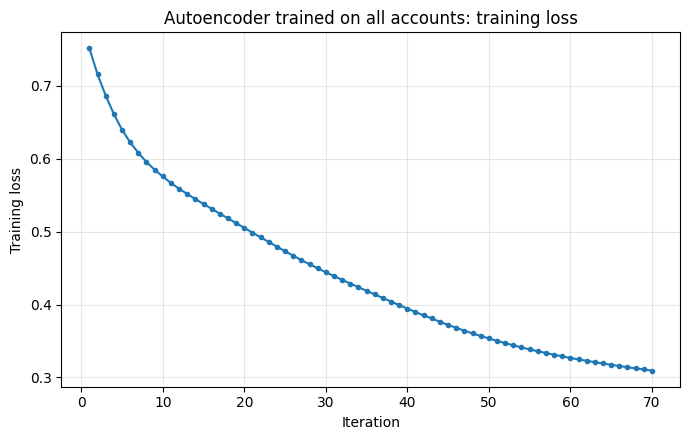
\includegraphics[width=0.75\textwidth]{results/output.png}
\caption{Training loss for the autoencoder trained on the full dataset.}
\label{fig:ae_all_loss}
\end{figure}
Figure~\ref{fig:ae_all_loss} shows the evolution of the reconstruction loss during training.
The loss decreases monotonically from approximately 0.75 to 0.31, indicating that the model
successfully learned to reconstruct the training observations.

However, a decreasing training loss alone does not imply that the learned representation
generalises well to unseen observations. Validation performance must also be examined.
\begin{figure}[H]
\centering
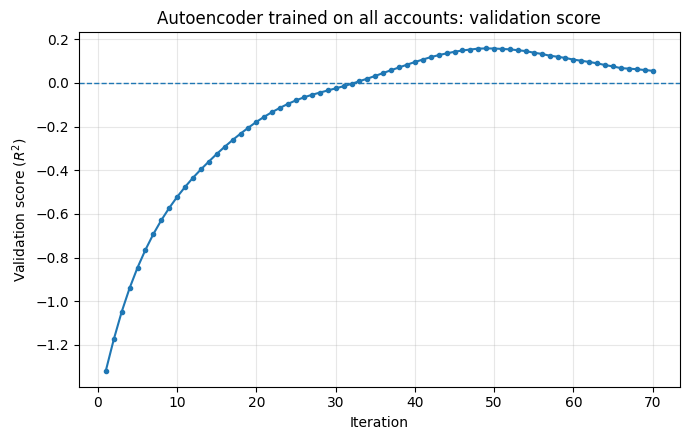
\includegraphics[width=0.75\textwidth]{results/output (1).png}
\caption{Validation score for the autoencoder trained on the full dataset.}
\label{fig:ae_all_val}
\end{figure}
Figure~\ref{fig:ae_all_val} presents the validation score reported by the
\texttt{MLPRegressor} implementation. The score corresponds to the coefficient of
determination ($R^2$) between the reconstructed and original feature vectors.

Although the validation score improves steadily throughout training, the best value obtained
is approximately 0.16. This indicates that only a relatively small proportion of the variation
in the validation observations is explained by the reconstructed outputs.

Consequently, the autoencoder exhibits limited reconstruction capability when trained on the
entire dataset. One possible explanation is that the training set contains both normal and
anomalous accounts, making it difficult for a single latent representation to accurately model
the dominant behaviour patterns.

To address this issue, a second experiment was conducted using only accounts belonging to
the large DBSCAN cluster identified before. Since this cluster contains the vast
majority of observations and is assumed to represent normal account behaviour, training the
autoencoder exclusively on this subset may allow the model to learn a cleaner representation
of normal activity patterns.

\subsection{Autoencoder Trained on Cluster 0}
The autoencoder trained only on DBSCAN Cluster 0 showed substantially improved reconstruction performance compared with the model trained on the full sample. The training loss decreased steadily from approximately \(0.737\) to \(0.149\), indicating that the network was able to reduce reconstruction error on the training data. At the same time, the validation score increased from a negative value to approximately \(R^2=0.704\), suggesting that the model also generalised well to unseen observations from Cluster 0.
\begin{figure}[H]
\centering
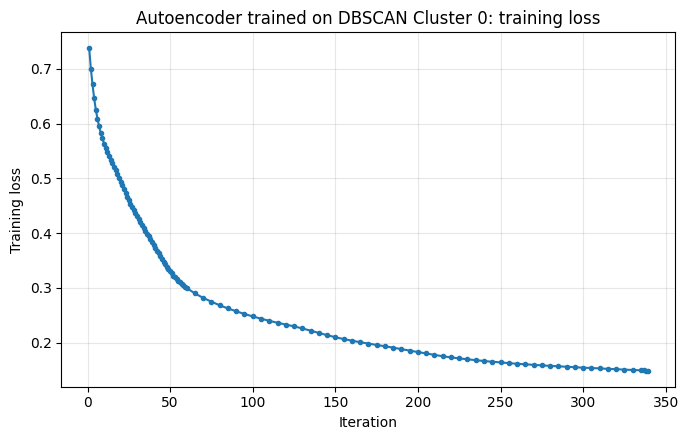
\includegraphics[width=0.75\textwidth]{results/output (2).png}
\caption{Training loss for the autoencoder trained on DBSCAN cluster 0.}
\label{fig:ae_all_val}
\end{figure}

\begin{figure}[H]
\centering
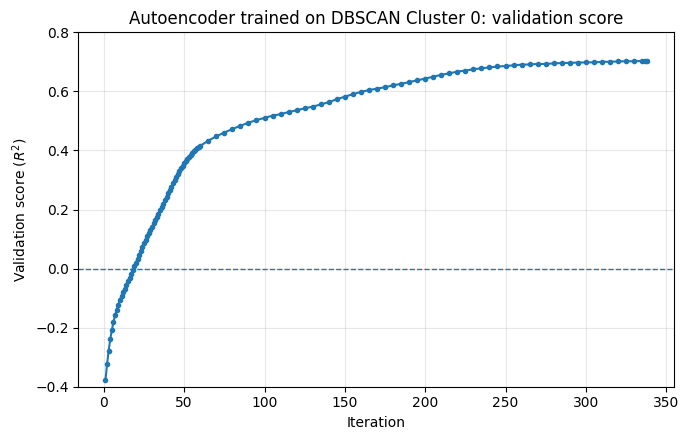
\includegraphics[width=0.75\textwidth]{results/output (4).png}
\caption{Training score for the autoencoder trained on DBSCAN cluster 0.}
\label{fig:ae_all_val}
\end{figure}
This supports the interpretation that Cluster 0 forms a more homogeneous approximation of normal account behaviour. In contrast, training the autoencoder on the full sample forced the model to reconstruct a more heterogeneous population, including noise observations, which led to much weaker validation performance. Therefore, the Cluster 0 autoencoder was used as the main reconstruction model for anomaly scoring.
\subsection{Manual Anomaly Injection Stress Test}

To further compare the anomaly sensitivity of the two autoencoder specifications, a manual anomaly injection experiment was conducted. A random 5\% of observations were selected from the sample and their feature values were modified to represent synthetic abnormal behaviours. This experiment was not intended as a formal evaluation of real money mule detection performance, since the injected observations are artificially constructed. Instead, it was used as a stress test to assess whether each autoencoder assigns high reconstruction errors to observations with clearly abnormal feature patterns.

Three types of synthetic anomalies were introduced. The first type represents mule-like pass-through behaviour. These observations were assigned high values for features such as the outgoing amount ratio, short-window drain ratio, near pass-through ratio, and one-in-many-out ratio. This corresponds to accounts where incoming funds are rapidly transferred out, often in amounts close to the incoming value. The second type represents burst behaviour, where transaction intensity and maximum-to-median amount ratios were increased. This captures accounts that suddenly become unusually active or receive unusually large transactions relative to their typical transaction size. The third type represents abnormal timing behaviour, where off-hours and weekend transaction ratios were increased, corresponding to accounts whose activity is concentrated outside normal working patterns.

After injecting the anomalies, both autoencoders were used to score all observations by reconstruction error. The top 20\% highest-error observations were then selected, and the number of injected anomalies recovered within this top-ranked group was recorded. The results are reported in Table~\ref{tab:ae_injection_test}.

\begin{table}[H]
\centering
\begin{tabular}{lcccc}
\hline
Model & Injected anomalies & Top 20\% size & Detected in top 20\% & Detection rate \\
\hline
AE trained on full sample & 91 & 365 & 28 & 30.8\% \\
AE trained on Cluster 0 & 91 & 365 & 60 & 65.9\% \\
\hline
\end{tabular}
\caption{Manual anomaly injection stress test for the two autoencoder models.}
\label{tab:ae_injection_test}
\end{table}

The autoencoder trained on Cluster 0 recovered 60 out of the 91 injected anomalies within the top 20\% reconstruction-error ranking, compared with 28 out of 91 for the autoencoder trained on the full sample. This indicates that the Cluster 0 autoencoder is substantially more sensitive to the injected abnormal behaviours. This result is consistent with the interpretation that Cluster 0 provides a cleaner approximation of normal account behaviour. Since the full-sample autoencoder is trained on a more heterogeneous population, including potentially noisy or unusual observations, it may learn to reconstruct a wider range of behaviours and therefore assign lower anomaly scores to some abnormal cases. In contrast, the Cluster 0 autoencoder learns a narrower normal reconstruction pattern, causing mule-like, burst, and timing anomalies to produce larger reconstruction errors.



\subsection{Supervised Learning Models}

In addition to the unsupervised anomaly detection methods, supervised baseline models were trained using the available confirmed mule labels. Confirmed mule accounts were treated as positive observations. Since verified non-mule labels were not available, the remaining sampled accounts were used as an unlabeled comparison group and were assigned label 0 for training purposes. Therefore, these models should be interpreted as label-informed baselines rather than fully validated mule-versus-non-mule classifiers.

Class weighting was used to account for the strong imbalance between the confirmed mule accounts and the unlabeled comparison group. The training set contained 72 confirmed mule observations and 1506 unlabeled observations, while the test set contained 20 confirmed mule observations and 320 unlabeled observations.

\subsubsection{Logistic Regression Results}

Logistic regression was used as an interpretable linear supervised baseline. The model estimates the log-odds of an account being a confirmed mule as a linear function of the engineered behavioural features. The classification report for the held-out test set is shown in Table~\ref{tab:logistic_classification_report}.

\begin{table}[H]
\centering
\begin{tabular}{lcccc}
\hline
Class & Precision & Recall & F1-score & Support \\
\hline
Unlabeled comparison group & 0.99 & 0.85 & 0.92 & 320 \\
Confirmed mule & 0.28 & 0.90 & 0.42 & 20 \\
\hline
Accuracy & \multicolumn{3}{c}{0.86} & 340 \\
Macro average & 0.63 & 0.88 & 0.67 & 340 \\
Weighted average & 0.95 & 0.86 & 0.89 & 340 \\
\hline
\end{tabular}
\caption{Classification report for the logistic regression supervised baseline.}
\label{tab:logistic_classification_report}
\end{table}

The logistic regression model achieved high recall for the confirmed mule class, correctly identifying 18 out of 20 confirmed mule accounts. However, its mule-class precision was relatively low at 0.28, meaning that a relatively large number of unlabeled accounts were also classified as mule-like. In the context of this study, these should not be interpreted as definitive false positives, since the unlabeled comparison group may contain hidden mule accounts. Instead, the result suggests that logistic regression is sensitive to mule-like behaviour but produces a broad suspicious-account ranking.
\begin{table}[H]
\centering
\begin{tabular}{lrr}
\hline
Feature & Coefficient & Absolute coefficient \\
\hline
drain\_ratio\_24h & 3.6739 & 3.6739 \\
outgoing\_txn\_ratio & -3.5964 & 3.5964 \\
outgoing\_amount\_ratio & -2.9349 & 2.9349 \\
one\_in\_many\_out\_24h\_ratio & 2.9615 & 2.9615 \\
mean\_median\_gap\_ratio & 1.5067 & 1.5067 \\
offhours\_ratio & 0.6305 & 0.6305 \\
log\_outgoing\_amount\_per\_span\_day & 0.4952 & 0.4952 \\
weekend\_ratio & 0.3982 & 0.3982 \\
max\_out\_method\_div\_after\_in\_1h & -0.1547 & 0.1547 \\
one\_in\_many\_out\_1h\_ratio & -0.1254 & 0.1254 \\
drain\_ratio\_1h & 0.0952 & 0.0952 \\
max\_out\_txn\_after\_in\_1h & 0.0831 & 0.0831 \\
near\_pass\_through\_24h\_ratio & 0.0708 & 0.0708 \\
txn\_per\_active\_day & -0.0396 & 0.0396 \\
near\_pass\_through\_1h\_ratio & 0.0195 & 0.0195 \\
max\_out\_txn\_after\_in\_24h & -0.0070 & 0.0070 \\
max\_median\_ratio & -0.0002 & 0.0002 \\
\hline
\end{tabular}
\caption{Logistic regression coefficients ranked by absolute coefficient magnitude.}
\label{tab:logistic_feature_importance}
\end{table}
The strongest positive coefficient was obtained for drain\_ratio\_24h, followed by one\_in\_many\_out\_24h\_ratio. This suggests that, within the fitted logistic regression model, accounts showing stronger 24-hour draining behaviour and one-in-many-out transfer patterns were assigned higher mule-risk scores. This is consistent with the expected behaviour of mule accounts, where incoming funds are rapidly forwarded to other destinations.

These negative coefficients should be interpreted cautiously. They do not necessarily imply that outgoing activity is protective. Instead, after more specific mule-behaviour variables such as drain\_ratio\_24h and one\_in\_many\_out\_24h\_ratio are included, the generic outgoing ratios may capture a different type of activity, such as normally active retail accounts with frequent outgoing payments but without clear draining behaviour.

In regression models, correlated predictors can make individual coefficient estimates less stable and may even lead to coefficient sign reversals or suppression effects 
\citep{vatcheva2016multicollinearity,ludlow2014suppressor}. Therefore, the coefficient 
ranking is used as a model-specific diagnostic of feature contribution rather than as formal 
evidence of individual feature significance.
\subsubsection{XGBoost Results}

XGBoost was used as a nonlinear supervised benchmark. Unlike logistic regression, it can capture threshold effects and interactions between behavioural features, which may be important in money mule detection because suspicious behaviour often depends on combinations of rapid drainage, pass-through ratios, transaction intensity, and unusual timing patterns. The classification report for the held-out test set is shown in Table~\ref{tab:xgboost_classification_report}.

\begin{table}[H]
\centering
\begin{tabular}{lcccc}
\hline
Class & Precision & Recall & F1-score & Support \\
\hline
Unlabeled comparison group & 0.98 & 0.99 & 0.99 & 320 \\
Confirmed mule & 0.79 & 0.75 & 0.77 & 20 \\
\hline
Accuracy & \multicolumn{3}{c}{0.97} & 340 \\
Macro average & 0.89 & 0.87 & 0.88 & 340 \\
Weighted average & 0.97 & 0.97 & 0.97 & 340 \\
\hline
\end{tabular}
\caption{Classification report for the XGBoost supervised baseline.}
\label{tab:xgboost_classification_report}
\end{table}

The XGBoost model achieved a more balanced performance than logistic regression. It identified 15 out of 20 confirmed mule accounts while producing only 4 positive predictions among the unlabeled comparison group. This resulted in a confirmed-mule precision of 0.79 and recall of 0.75. Therefore, XGBoost provided a stronger supervised predictive ranking, especially in terms of precision.
\begin{table}[H]
\centering
\begin{tabular}{lr}
\hline
Feature & Importance \\
\hline
txn\_per\_active\_day & 0.2192 \\
drain\_ratio\_24h & 0.1212 \\
log\_outgoing\_amount\_per\_span\_day & 0.0794 \\
outgoing\_txn\_ratio & 0.0737 \\
max\_out\_txn\_after\_in\_1h & 0.0481 \\
mean\_median\_gap\_ratio & 0.0457 \\
outgoing\_amount\_ratio & 0.0445 \\
one\_in\_many\_out\_24h\_ratio & 0.0419 \\
max\_median\_ratio & 0.0410 \\
offhours\_ratio & 0.0407 \\
drain\_ratio\_1h & 0.0382 \\
max\_out\_method\_div\_after\_in\_1h & 0.0371 \\
weekend\_ratio & 0.0368 \\
max\_out\_txn\_after\_in\_24h & 0.0336 \\
near\_pass\_through\_24h\_ratio & 0.0302 \\
near\_pass\_through\_1h\_ratio & 0.0292 \\
\hline
\end{tabular}
\caption{XGBoost "Gain" feature importance values.}
\label{tab:xgboost_feature_importance}
\end{table}
\begin{figure}[htbp]
    \centering
    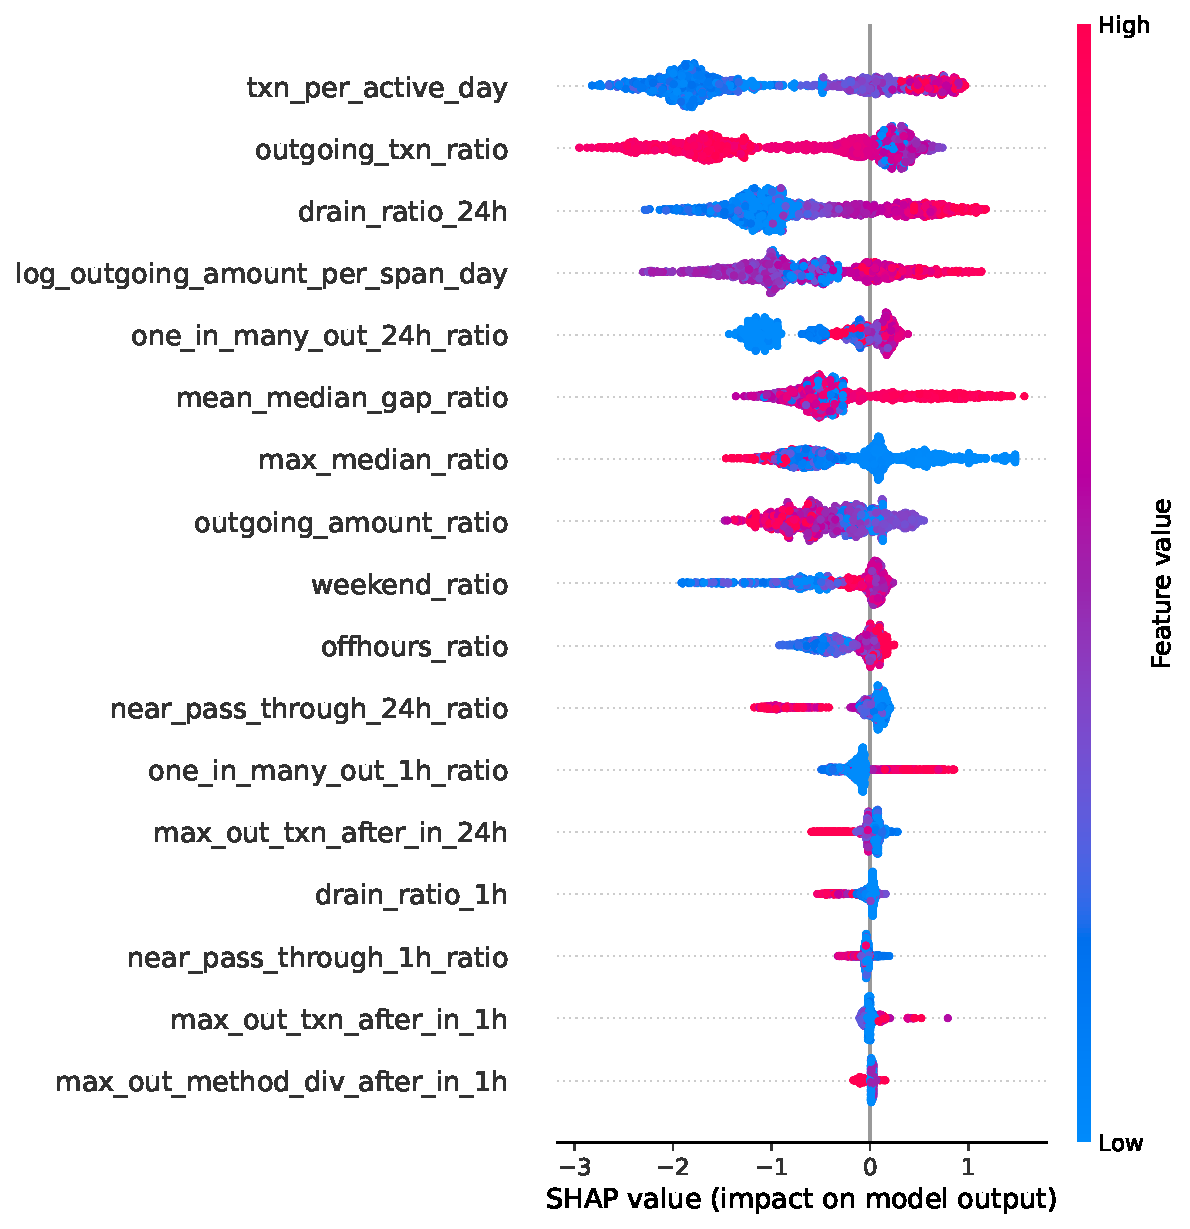
\includegraphics[width=0.55\textwidth]{methods/shap_summary_plot.pdf}
    \caption{SHAP summary plot for the XGBoost classifier.}
\end{figure}
Figure 6.5 presents the SHAP summary plot for the XGBoost classifier. The features are ranked by their mean absolute SHAP values, so variables appearing higher in the plot have a larger average impact on the model output. Each point represents one observation. The horizontal position shows the SHAP value, where positive values push the prediction towards the confirmed mule class and negative values push it towards the unlabeled comparison class. The colour indicates the feature value, with red corresponding to high feature values and blue corresponding to low feature values.

The most influential variable was \texttt{txn\_per\_active\_day}, indicating that transaction frequency per active day had the largest average impact on the XGBoost predictions. Higher values of this feature generally pushed the model output towards the confirmed mule class, suggesting that the model associated higher transaction intensity with greater mule risk. However, this variable is not mule-specific and may also capture generally active retail behaviour.

More mule-specific behavioural features also appeared among the most important variables. High values of \texttt{drain\_ratio\_24h} generally produced positive SHAP values, meaning that stronger 24-hour draining behaviour increased the predicted mule-risk score. Similarly, high values of \texttt{one\_in\_many\_out\_24h\_ratio} tended to push predictions towards the confirmed mule class. These patterns are consistent with the expected behaviour of money mule accounts, where incoming funds are rapidly forwarded onwards, sometimes through multiple outgoing transfers.

By contrast, \texttt{outgoing\_txn\_ratio} showed a negative effect for high feature values, with high values tending to push the prediction away from the confirmed mule class. This should not be interpreted as evidence that outgoing activity is inherently non-suspicious. Rather, after accounting for more targeted mule-behaviour variables such as draining and one-in-many-out behaviour, generic outgoing transaction activity may capture normally active retail behaviour without clear rapid forwarding patterns.

Overall, the SHAP analysis suggests that the XGBoost classifier relied on both general activity intensity and more specific mule-behaviour indicators. The most business-relevant positive drivers were \texttt{drain\_ratio\_24h} and \texttt{one\_in\_many\_out\_24h\_ratio}, while the importance of \texttt{txn\_per\_active\_day} indicates that the model also learned differences in overall transaction activity between confirmed mule accounts and the unlabeled comparison group.
\subsubsection{Comparison of Supervised Models}

A summary comparison of the two supervised baselines is given in Table~\ref{tab:supervised_summary}. Since the positive class is rare, PR-AUC is particularly informative because its random baseline corresponds approximately to the positive-class prevalence.

\begin{table}[H]
\centering
\begin{tabular}{lccccc}
\hline
Model & ROC-AUC & PR-AUC & Mule precision & Mule recall & Mule F1-score \\
\hline
Logistic regression & 0.936 & 0.552 & 0.28 & 0.90 & 0.42 \\
XGBoost & 0.946 & 0.811 & 0.79 & 0.75 & 0.77 \\
\hline
\end{tabular}
\caption{Summary comparison of supervised baseline models on the held-out test set.}
\label{tab:supervised_summary}
\end{table}

Overall, XGBoost achieved stronger predictive performance, particularly in terms of PR-AUC and mule-class precision. Logistic regression, however, remained useful as an interpretable baseline. Its largest coefficients were associated with engineered mule-behaviour features such as drain ratios, one-in-many-out ratios, outgoing transaction ratios, outgoing amount ratios, and near pass-through measures. This suggests that the supervised signal learned by the linear model is closely aligned with the intended behavioural definition of mule activity. In contrast, XGBoost used both mule-specific flow features and broader activity-intensity features, such as transactions per active day. This indicates that XGBoost captured a more complex nonlinear risk pattern, while logistic regression provided a clearer feature-level interpretation. 

Both models shown that drain ratio is a very important feature which provides strong signal, which is also the most computational heavy feature among all. This finding also aligned with business level interpretation. 

The supervised results should still be interpreted cautiously. The negative class consists of unlabeled accounts rather than verified non-mules, so the reported metrics depend on the temporary assumption that unlabeled accounts can be treated as negatives for baseline training and evaluation. For this reason, the supervised models are best understood as label-informed ranking methods rather than definitive classifiers of money mule behaviour.
